\newpage
\section{Podręcznik użytkownika}  %6
%Opis jak używać programu. Mogą być z zrzut ekranu razem z opisem. 
\subsection{Menu główne}
Menu główne w aplikacji "Operacja Kooperacja"~ zawiera pierwszą zagadkę w grze. Jest nią duży czerowny przycisk z napisem "CLICK HERE". Po wciśnięciu tego przycisku aplikacja zamyka się natomiast przyciisk z "żarówką"~ pozwala nam przejść dalej.
	\begin{figure}[!htb]
	\begin{center}
		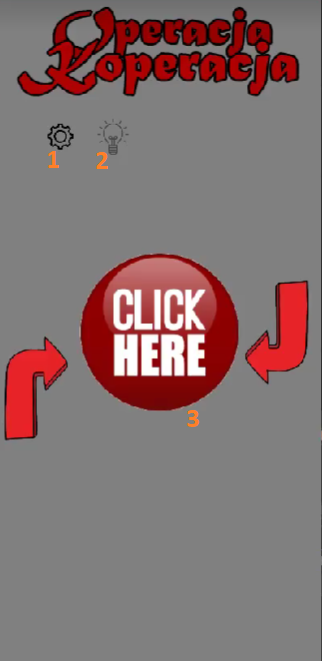
\includegraphics[width=8cm]{rys/opis1.png}
		\caption{Menu Główne}
		\label{rys:rysunek001}
	\end{center}
\end{figure}

\begin{enumerate}
	\item Przycisk pozwalający nam przejść do ustawień, 
	\item Przycisk pozwalający nam przejść do właściwego menu głównego,
	\item Przycisk ten wyłącza aplikacje, 
\end{enumerate}

	\begin{figure}[!htb]
	\begin{center}
		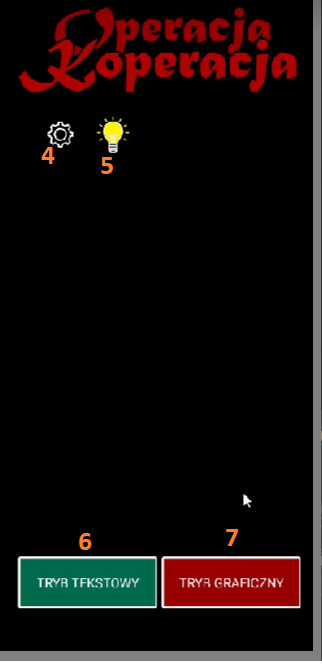
\includegraphics[width=8cm]{rys/opis3.png}
		\caption{Menu Główne v2}
		\label{rys:rysunek001}
	\end{center}
\end{figure}


\begin{enumerate}
	\setcounter{enumi}{3}
	\item Przycisk pozwalający nam przejść do ustawień, 
	\item Przycisk pozwalający nam przejść do poprzedniego menu głównego,
	\item Przycisk ten pozwala nam wybrać tryb tekstowy jako nasz tryb gry,
	\item Przycisk ten pozwala nam wybrać tryb graficzny jako nasz tryb gry.
\end{enumerate}

\subsection{Tryb tekstowy}
Po wejściu w tryb teksotwy ukazuje nam się takie okno jak na rys 6.3. Tutaj wprowadzamy kod w odpowiednim miejscu, który pozwoli nam zobaczyć podpowiedzi do danej zagadki. Kod jest widoczny w trybie graficznym razem z opisem zagadki w~komunikacie przed rozpoczęciem próby rozwiązania zagadki.
	\begin{figure}[!htb]
	\begin{center}
		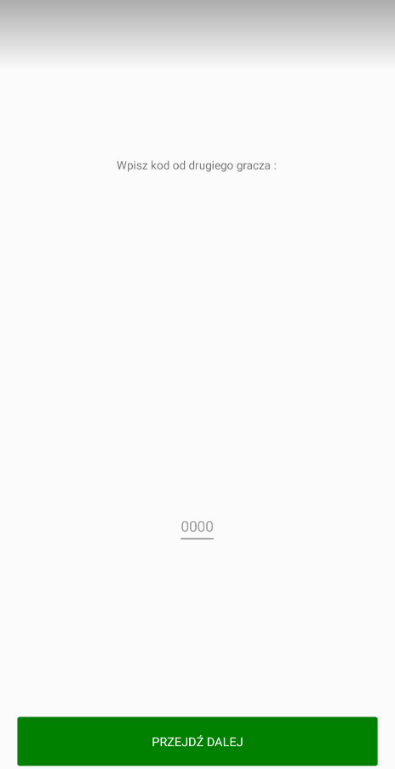
\includegraphics[width=8cm]{rys/tekstowy0.png}
		\caption{Tryb tekstowy}
		\label{rys:rysunek001}
	\end{center}
\end{figure}

\subsection{Labirynt}
Po wybraniu graficznego trybu gry zostajemy przeniesieni do pierwszej zagadki, którą jest labirynt. Na początku dostajemy informacje o zagadce jak i kod do trybu tekstowego dla naszego partnera. Ta zagadka polega na doprowadzeniu postaci (pomarańczowego kwadratu) do wyjścia. Osoba w trybie graficznym widzi kilka wersji labiryntu i musi wybrać właściwy na podstawie informacji jakie dostanie od partnera, po czym musi poprowadzić osobę z trybu graficznego do wyjścia. Każde wejście w ściane kończy się utratą życia i zresetowaniem pozycji postaci.
\\
\\
\\
\\
	\begin{figure}[!htb]
	\begin{center}
		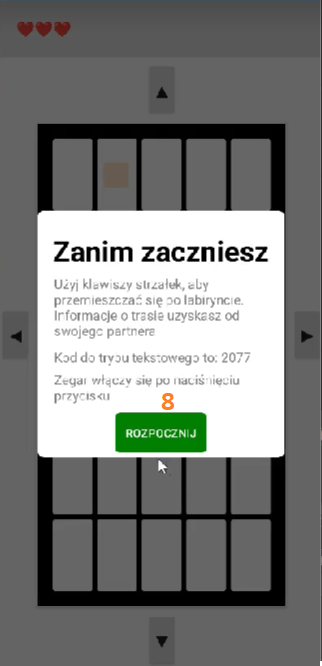
\includegraphics[width=8cm]{rys/opis2.png}
		\caption{Komunikat (Labirynt)}
		\label{rys:rysunek001}
	\end{center}
\end{figure}

\begin{enumerate}
	\setcounter{enumi}{7}
	\item Przycisk pozwalający nam rozpocząć grę,
\end{enumerate}

	\begin{figure}[!htb]
	\begin{center}
		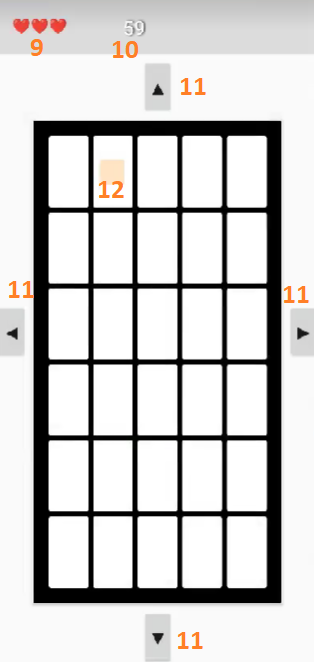
\includegraphics[width=8cm]{rys/opis4.png}
		\caption{Labirynt}
		\label{rys:rysunek001}
	\end{center}
\end{figure}

\begin{enumerate}
	\setcounter{enumi}{8}
	\item Licznik żyć (Zaczynamy mając 3 życia, w momencie utraty ostatniego przegrywamy),
	\item Timer (Pokazuje ile czasu mamy na daną zagadkę),
	\item Przyciski pozwalające poruszać naszą "postacią",
	\item Postać, którą sterujemy.
\end{enumerate}

	\begin{figure}[!htb]
	\begin{center}
		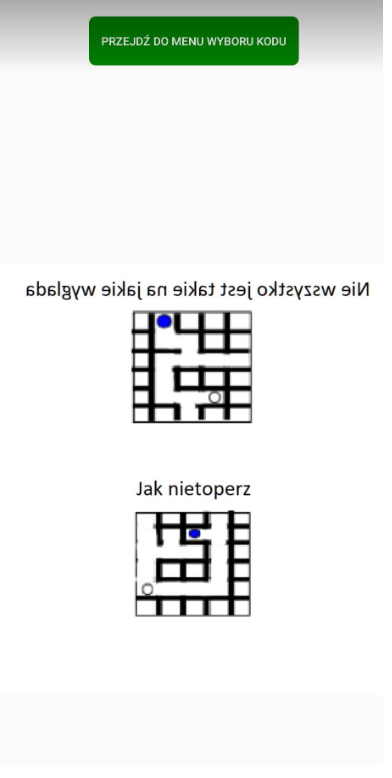
\includegraphics[width=8cm]{rys/tekstowy1.png}
		\caption{Tryb tekstowy (Labirynt)}
		\label{rys:rysunek001}
	\end{center}
\end{figure}
\hspace{-0.60cm}Jak widać na rys 6.6 tryb teksowy do zagadki "Labirynt"~ przedstawia możliwe rozłożenia labiryntu ale w tym trybie też są zagadki. Dla przykładu pierwsze rozłożenie labiryntu jest odbite lustrzanie od właściwego a drugie jest do góry nogami.
\subsection{Literaki}
Po przejściu "Labiryntu"~ zostajemy przeniesieni do kolejnej zagadki, którą są "Literaki". Podobnie jak w przypadku poprzedniej zagadki dostajemy opis tego co mamy zrobić i kod do trybu tekstowego. W tej zagadce chodzi o to, żeby razem z partnerem z trybu tektowego ustalić jakie hasło pozwoli nam przejść dalej. Gracz w trybie teksowym widzi dostępne słowa natomiast gracz w trybie graficznym musi za pomocą strzałek zmieniać litery na odpowiednich polach dopóki nie powstanie z nich jedno z tych słów. Liczba liter przypadająca na każde pole jest ograniczona.

	\begin{figure}[!htb]
	\begin{center}
		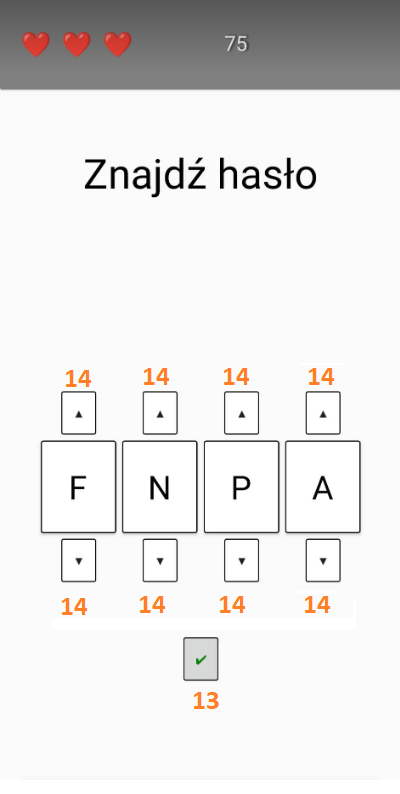
\includegraphics[width=8cm]{rys/opis6.png}
		\caption{Literaki}
		\label{rys:rysunek001}
	\end{center}
\end{figure}

\begin{enumerate}
	\setcounter{enumi}{12}
	\item Przycisk, którym zatwierdzamy hasło,
	\item Przyciski pozwalające na zmiane litery na odpowiednim miejscu.
\end{enumerate}

	\begin{figure}[!htb]
	\begin{center}
		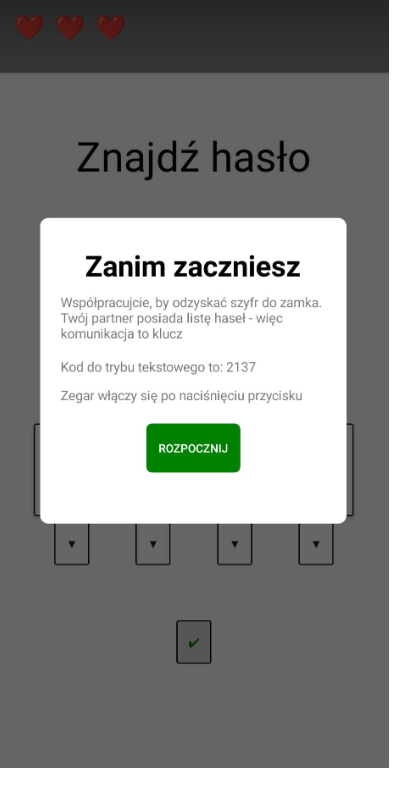
\includegraphics[width=8cm]{rys/opis8.png}
		\caption{Komunikat (Literaki))}
		\label{rys:rysunek001}
	\end{center}
\end{figure}

	\begin{figure}[!htb]
	\begin{center}
		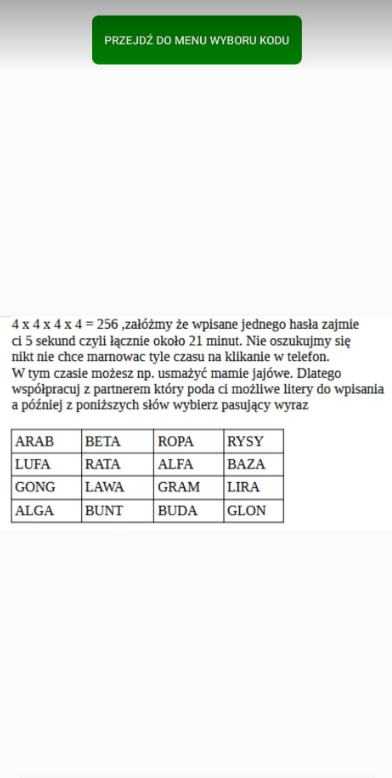
\includegraphics[width=8cm]{rys/tekstowy2.png}
		\caption{Tryb tekstowy (Literaki)}
		\label{rys:rysunek001}
	\end{center}
\end{figure}
\hspace{-0.60cm}Tryb tekstowy dla zagadki "Literaki" (rys 6.9) zawiera tabelę możliwych słow, autorski opis dlaczego nie warto próbować na siłę wpisywać hasła i dlaczego lepiej jest współpracować.
\\
\\
\\
\\
\\
\\
\\
\\
\\
\subsection{Kod Morsa}
Po ukończeniu "Literaków"~ zostajemy przeniesieni do zagadki, która nazywa się "Kod Morsa". Podobnie jak w przypadku poprzednich zagadek dostajemy opis zadań i kod do trybu tekstowego (rys 6.10). Ta zagadka jest podobna do ~"Literaków" z~ jedną różnicą. Gracz w tybie tekstowym ma opisane słowa za pomocą kodu morsa. Gracz trybu graficznego dostaje, poprzez włączanie i wyłącznie latarki, długie i~krótkie sygnały, które po skonsultowaniu z partnerem pozwolą odgadnąć hasło. 
\\
\\
	\begin{figure}[!htb]
	\begin{center}
		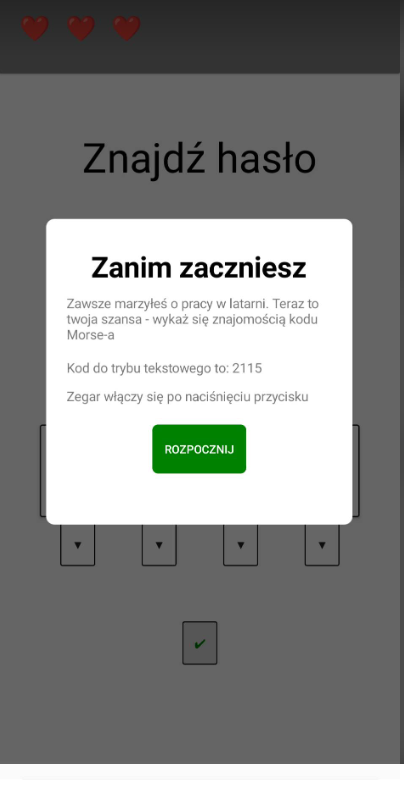
\includegraphics[width=8cm]{rys/opis7.png}
		\caption{Komunikat (Kod Morsa)}
		\label{rys:rysunek001}
	\end{center}
\end{figure}
	\begin{figure}[!htb]
	\begin{center}
		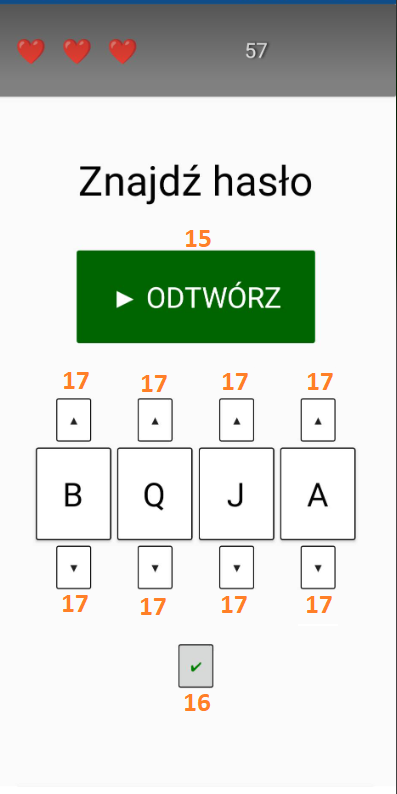
\includegraphics[width=8cm]{rys/opis5.png}
		\caption{Kod Morsa}
		\label{rys:rysunek001}
	\end{center}
\end{figure}

\begin{enumerate}
	\setcounter{enumi}{14}
	\item Przycisk, którym odtwarzamy kod morsa za pomocą latarki,
	\item Przycisk, którym zatwierdzamy hasło,
	\item Przyciski pozwalające na zmiane litery na odpowiednim miejscu.
	\\
	\\
	\\
	\\
	\\
	\\
\end{enumerate}

	\begin{figure}[!htb]
	\begin{center}
		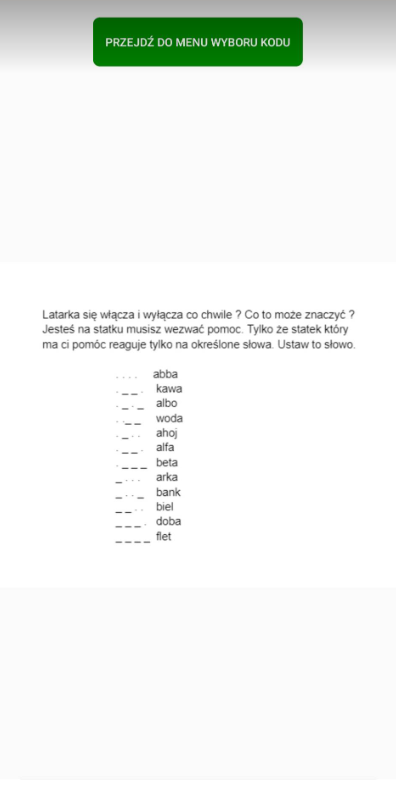
\includegraphics[width=8cm]{rys/tekstowy3.png}
		\caption{Tryb tekstowy (Kod Morsa)}
		\label{rys:rysunek001}
	\end{center}
\end{figure}
\hspace{-0.60cm}W trybie tekstowym (rys 6.12) dla trybu "Kod Morsa"~ są rozpisane słowa wraz z ich odpowiednikiem w kodzie. Kropka oznacza sygnał krótki a kreska sygnał długi.
\\
\\
\\
\\
\\
\subsection{Kolorki}
Po ukończeniu "Kodu Morsa"~ zostajemy przeniesieni do zagadki, która nazywa się "Kolorki". Podobnie jak w przypadku poprzednich zagadek dostajemy opis zadań i kod do trybu tekstowego (rys 6.13). Ta zagadka polega na odtworzeniu sygnału, który zostaje nam wyświetlony. W trybie tekstowym mamy opisane, przycisk w~jakim kolorze mamy nacisnąć po otrzymaniu konkretnego koloru. Gracz w trybie graficznym musi powtórzyć otrzymany kod. Początkowo jeden przycisk stopniowo zwiększając ich liczbę do pięciu.
\\
	\begin{figure}[!htb]
	\begin{center}
		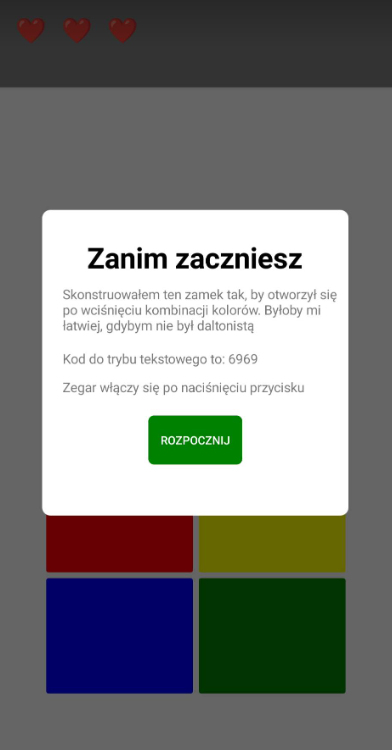
\includegraphics[width=8cm]{rys/opis9.png}
		\caption{Komunikat (Kolorki)}
		\label{rys:rysunek001}
	\end{center}
\end{figure}

	\begin{figure}[!htb]
	\begin{center}
		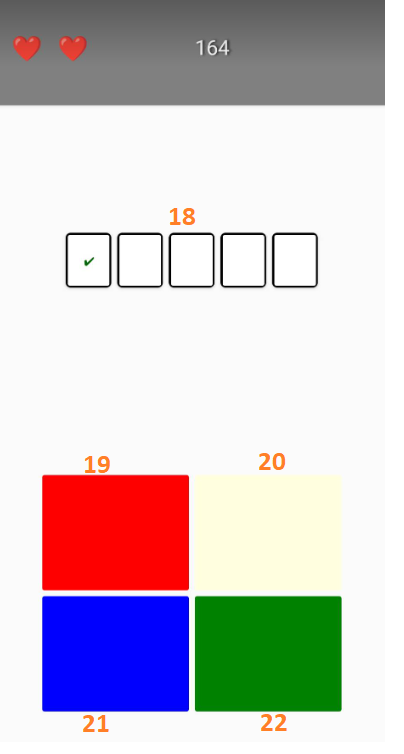
\includegraphics[width=8cm]{rys/opis10.png}
		\caption{Kolorki}
		\label{rys:rysunek001}
	\end{center}
\end{figure}

\begin{enumerate}
	\setcounter{enumi}{17}
	\item Licznik, który pokazuje ile jeszcze kolorów nam zostało do zgadnięcia,
	\item Przycisk, który odpowiada za określony kolor,
	\item Przycisk, który został wyróżniony i gracz musi kliknąć jego odpowiednik na podstawie informacji z trybu tekstowego,
	\item Przycisk, który odpowiada za określony kolor,
	\item Przycisk, który odpowiada za określony kolor.
	\\
	\\
\end{enumerate}

	\begin{figure}[!htb]
	\begin{center}
		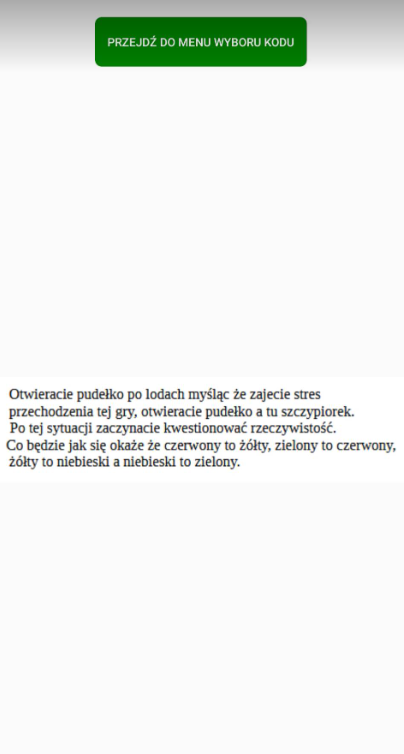
\includegraphics[width=8cm]{rys/tekstowy4.png}
		\caption{Tryb tekstowy (Kolorki)}
		\label{rys:rysunek001}
	\end{center}
\end{figure}
\hspace{-0.60cm}W trybie tekstowym dla tej zagadki (rys. 6.15) jest krótka historyjka i opis, który kolor ma kliknąć gracz w trybie graficznym jeżeli wyświetli się konkretny. Dla przykładu jeżeli gracz z trybu graficznego zobaczy wyróżniony zielony kolor musi wciisnąć czerwony przycisk
\\
\\
\\
\\
\\
\\
\subsection{Wielki Przycisk}
Po ukończeniu "Kolorków"~ zostajemy przeniesieni do zagadki, która nazywa się "Wielki Przycisk". Podobnie jak w przypadku poprzednich zagadek dostajemy opis zadań i kod do trybu tekstowego (rys 6.16). Ta zagadka polega na przytrzymaniu palca na przycisku przez określony czas zaczynając od określonego czasu na timerze. Wszysko zostało opisane w trybie tekstowym.
\\
\\
\\
\\
\\
	\begin{figure}[!htb]
	\begin{center}
		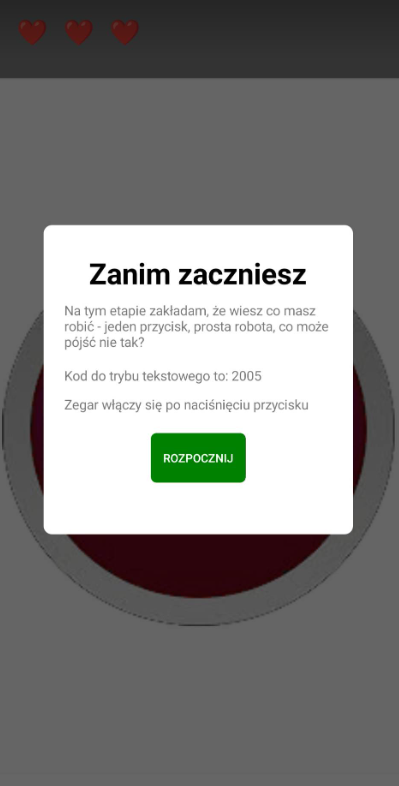
\includegraphics[width=8cm]{rys/opis11.png}
		\caption{Komunikat (Wielki Przycisk)}
		\label{rys:rysunek001}
	\end{center}
\end{figure}
\begin{enumerate}
	\setcounter{enumi}{22}
	\item Wielki Przycisk, który mamy przytrzymać przez określoną liczbę sekund.
	\\
	\\
	\\
	\\
	\\
	\\
	\\
	\\
	\\
\end{enumerate}
	\begin{figure}[!htb]
	\begin{center}
		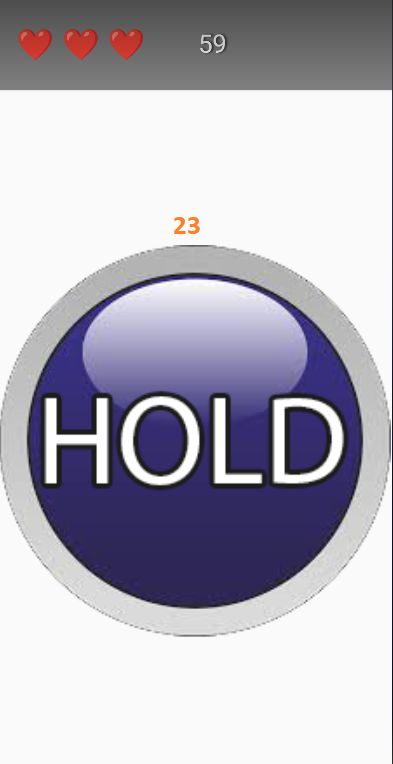
\includegraphics[width=8cm]{rys/opis12.png}
		\caption{Wielki Przycisk}
		\label{rys:rysunek001}
	\end{center}
\end{figure}

	\begin{figure}[!htb]
	\begin{center}
		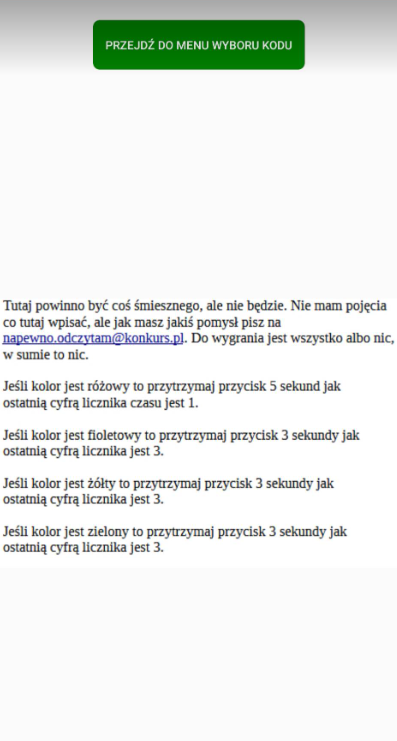
\includegraphics[width=8cm]{rys/tekstowy5.png}
		\caption{Tekstowy (Wielki Przycisk)}
		\label{rys:rysunek001}
	\end{center}
\end{figure}
\hspace{-0.60cm}W trybie tekstowym dla zagadki "Wielki Przycisk"~(rys 6.18) mamy napisane ile sekund i przy jakim czasie na timerze mamy przytrzymać przycisk.
\\
\\
\\
\\
\\
\\
\\
\\
\subsection{Tabela wyników}
Po przejściu wszyskich zagadek automatycznie przechodzimy do tabeli wyników i w odpowiednim polu wpisujemy swoje imie (rys 6.19). Po podaniu imienia nasz wynik zostaje dodany do tabeli wyników i zestawiony z innymi (rys 6.20).

	\begin{figure}[!htb]
	\begin{center}
		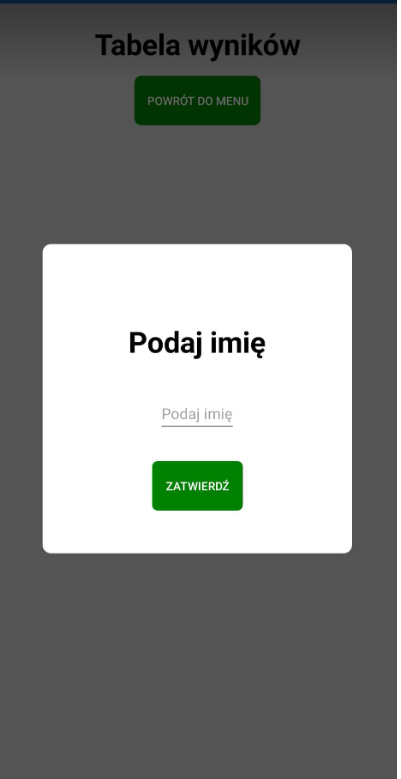
\includegraphics[width=8cm]{rys/opis13.png}
		\caption{Tabela wyników (Podaj imie)}
		\label{rys:rysunek001}
	\end{center}
\end{figure}

	\begin{figure}[!htb]
	\begin{center}
		
\includegraphics[width=8cm]{rys/opis14.png}
		\caption{Tabela wyników}
		\label{rys:rysunek001}
	\end{center}
\end{figure}
